\documentclass[11pt,a4paper]{scrartcl}
\usepackage[utf8]{inputenc}
\usepackage[english,brazil,brazilian]{babel}
\usepackage{amsmath}
\usepackage{amsfonts}
\usepackage{amssymb}
\usepackage{graphicx}
\usepackage{todonotes}

\newcommand{\unit}[1]{\ensuremath{\, \mathrm{#1}}}

\title{Processamento Digital de Sinais\\ Eletrocardiograma + HIL}
\author{Rafael Corsi}


\begin{document}
\maketitle

\section{ECG}

Eletrocardiograma (ECG ou EKG) é o histórico das atividades elétricas do corpo (coração) amostradas através de eletrodos na superfície do corpo. Esses dados são utilizados para extração de informações uteis na analise clinica do paciente. Intervalo de tempo entre pulsos, suas formas e orientações (Fig. \ref{fig:parametros:ecg}) representam fenômenos fisiológicos que ocorrem no coração e nos sistemas nervosos.

\begin{figure}[!ht]
\centering
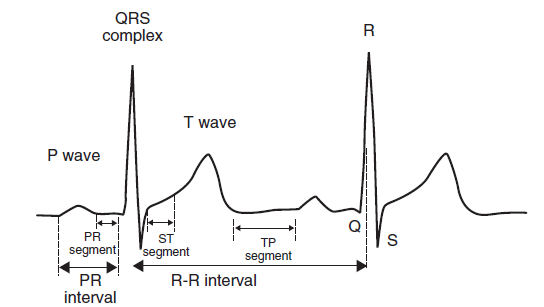
\includegraphics[width=0.5\textwidth]{figs/ecg.png}
\caption{Parâmetros de um ECG}
\label{fig:parametros:ecg}
\end{figure}

Devido a baixa relação sinal/ruido, interferências de outros sinais (movimentos do paciente, eletrônica entre outros) uma das etapas mais importantes do sistema é a filtragem do sinal. 

\section{HIL}

Hardware-in-the loop (HIL) é um técnica de simulação em tempo real (onde a taxa de amostragem é respeitada) capaz de simular sistemas dinâmicos e suas interfaces externas, simulando assim uma planta real. Muito utilizado para prototipagem de sistemas de controle onde o acesso ao sistema real não é possível (ex. planta nuclear, satélites \ldots) ou em estágios iniciais do desenvolvimento. 

Um HIL pode ser desenvolvido utilizando o software \textit{Simulink} em conjunto com a placa de aquisição DAQ 6251 (\textit{Data Acquisition}) (Elvis).

\section{Desafio}

Desenvolver um ECG embarcado que colete os dados de um eletrodo (rodando no HIL) , filtre o sinal e detecte a frequência cardíaca do paciente.

\begin{figure}[!ht]
\centering
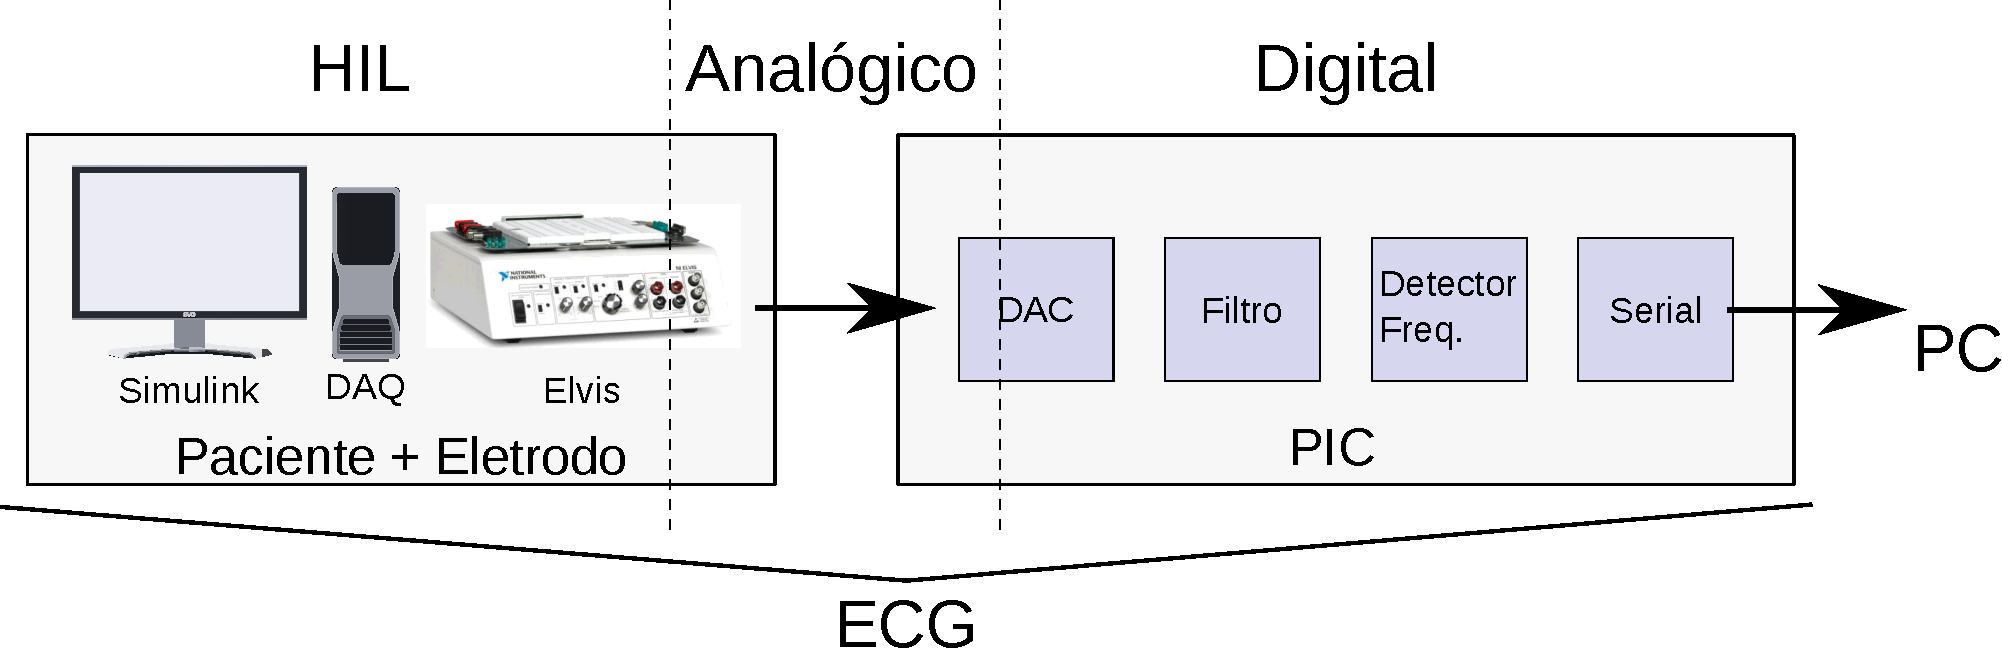
\includegraphics[width=1\textwidth]{figs/esquema.pdf}
\caption{Sistema proposto}
\label{fig:esquema}
\end{figure}

\begin{figure}[!ht]
\centering
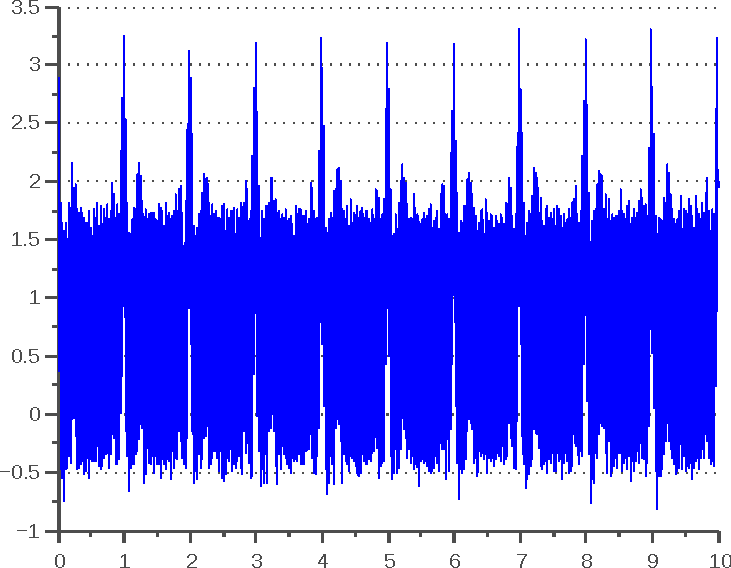
\includegraphics[width=0.5\textwidth]{figs/ECG.pdf}
\caption{Sinal com ruido}
\label{fig:ruido}
\end{figure}

\subsection{Etapas Matlab} \label{etapa:matlab}

\begin{enumerate}
	\item Implementar o ECG e verificar o sinal com um osciloscópio (\textbf{ecg-modelo-hil.mdl})
	\item Plotar o espectro do sinal, analisando os ruídos  (\textbf{ecg-main.m})
	\item Projetar um filtro para o sistema e verificar sua eficiência no sinal do item 2 (\textbf{ecg-modelo-i.mdl}). 
		\begin{itemize}
			\item FIR ou IIR ?
			\item Pensando já na etapa embarcada, qual o melhor formato de varáveis a trabalhar ? (int, float, \ldots) e qual o efeito do truncamento na resposta do filtro ? Podemos usar um filtro com ordem muito grande ?
		\end{itemize}
	\item Discretizar o filtro \label{filtro:discreto}
\end{enumerate}

\subsection{Etapas Embarcado}

\begin{enumerate}
	\item Coletar os dados analógicos (qual taxa de amostragem ?)
	\item Enviar os dados coletados via serial (para debug)
	\item Implementar o filtro desenvolvido em \ref{etapa:matlab} item \ref{filtro:discreto} (\textbf{filtro.c e filtro.h})
	\item Detectar frequência cardíaca e plotar o dado no LCD;
	\item Validar o resultado
\end{enumerate}

\subsection{Arquivos}

Os seguintes arquivos serão fornecidos:

\begin{itemize}
	\item \textbf{ecg-modelo-hil.mdl :} Modelo do simulink do ECG para HIL;
	
	\begin{itemize}
		\item  A porta utilizada é a \textit{DAC 0}
	\end{itemize}
	
 \item \textbf{ecg-modelo-i.mdl :} Modelo no simulink para simulação com proposta de filtro FIR;
	 
	\item \textbf{ecg-dado.mat :} Workspace do matlab que contém as variáveis utilziadas pelo simulink;
	
	\begin{itemize}
		\item \textbf{Ts :} Taxa de amostragem;
		\item \textbf{dado :} Estrutura contendo o sinal;
		\item \textbf{simout :} Estrutura  contendo o sinal simulado;
	\end{itemize}
	
	\item \textbf{ecg-main.m :} Script para inicialização e analise do ECG; 
	
	\item \textbf{filtro.c :} Template em \textit{C} para implementação de um filtro FIR;
	\item\textbf{filtro.h :} Parâmetros do filtro.
	
\end{itemize}



\end{document}